%!TEX root = ../template.tex
%%%%%%%%%%%%%%%%%%%%%%%%%%%%%%%%%%%%%%%%%%%%%%%%%%%%%%%%%%%%%%%%%%%
%% methodology.tex
%% NOVA thesis document file
%%
%% Chapter with Methodology
%% (older Previous Work)
%%%%%%%%%%%%%%%%%%%%%%%%%%%%%%%%%%%%%%%%%%%%%%%%%%%%%%%%%%%%%%%%%%%

%REVIWED IN 2022/03/30
%COMPLETED IN 2022/03/30

\typeout{NT FILE methodology.tex}

\chapter{Methodology}
\label{cha:introduction}

\section{Introduction} 
\label{sub:if_you_use_this_template} 
In order to advance, and better prepare the study of this thesis, a specific study on CGI RMS data and research was developed, to get a starting point on the variables data and algorithms.

As presented before, this study will use a data-driven based method that involves less restriction in knowing all the details of the underlying fault process and the technical knowledge of all the components \cite{OLD_19_WIND}. With the large amount of historical data that is available in the CGI RMS, all the conditions are reunited to start developing the work with this method.

Since our goal is to build an generic experiment in Azure Machine Learning Studio that may be used as a foundation for the Failure Prediction tool, and due to the limitations of the signals that we have available and the built-in modules available in Azure Machine Learning Studio, we have to analyze our literature and confront with the modules available in order to obtain the best experiment possible to build the best model to predict the failures of the wind turbines that are being studied.

% DEPRECATED
%With several studies like [OLD 2] \cite{40_WIND} \cite{OLD_36_SOLAR}, we can understand %and select the machine learning algorithms that should be used and %compared to obtain the best model for failure prediction.

%these studies [XXX] analyzed several fault types, with major highlight on %(TO SEE COM REFERENCIAS). The signals that were used on these studies, %depend on the data that each one have available, but in all of them %[XXXX] there were used general data like XXXX. In [Y], vibration data %were used. These types of signals are one of the best signals to %understand possible failures as said by CGI experts. In [Z] were also %used these signals XXX.


\section{Data Structure} 
\label{sub:if_you_use_this_template} 

Following the previous knowledge obtained with RMS CGI, the data model presented in Figure 5.1 and Figure 5.2, provides a global overview of the classification of an event into a failure of a certain type, and of how data from assets are obtained and stored.

Before all the data acquisition begins, the client (owner of the parks) provides all the information needed to monitor the complete wind park. The most important data entities for this thesis are:

\begin{enumerate}
    \item 
Information about each wind park and their respective wind turbines, that we call assets of the park. Each asset has a determined manufacturer, model, and controller.
    \item
Components, which are the basic units that forms each wind turbine and that allow us to understand where a certain event occurs.
    \item
Signals, that exist in each asset or in the park. These signals provide us different information, like the active power for example or the wind speed.
    \item
Faults, that allow us to understand the cause of a failure and the component where it occurs. It is going to be one of the main entities for this thesis.
    \item
Statuses, that allows us to associate to each asset their status and acknowledge the status associated with an event. The downtimes presented before, may be associated to one or more statuses.
    \item
Budgets, that are used as monthly expectations that the park owners have on their assets in different type of measures (like production, ratio of performance). Allied with KPIs, allow to better under-stand the performance of the assets.
    \item
Key Performance Indicators (KPIs), that are calculations over signals that allow for a quicker understatement of the performance of the wind turbines. May allied more than one source of information (like signals or budgets) to provide a final value that directly indicate the performance of a wind turbine or park.
\end{enumerate}

Other data that is provided to us, including some classifications and indicators that the system already have in its basis, are adapted to the specification of each client.

In terms of the process of data acquisition, it involves all the entities represented in Figure 5.1. It begins with an event, registered with a certain state allied. Events are one of the most basic units registered in our system. RMS have a state machine, that uses these events and static data presented before like faults and states, allowing us to calculate the energy loss, duration, and number of events that occur in a certain time interval, and present the downtime of an asset and the classification of that downtime, meaning, the motive for that failure to occur. Each event is counted as one until a change of it state occurs, meaning that a single event may last for days (for example, for an event that states that a wind turbine is running).

\begin{figure}[htbp]
	\centering
	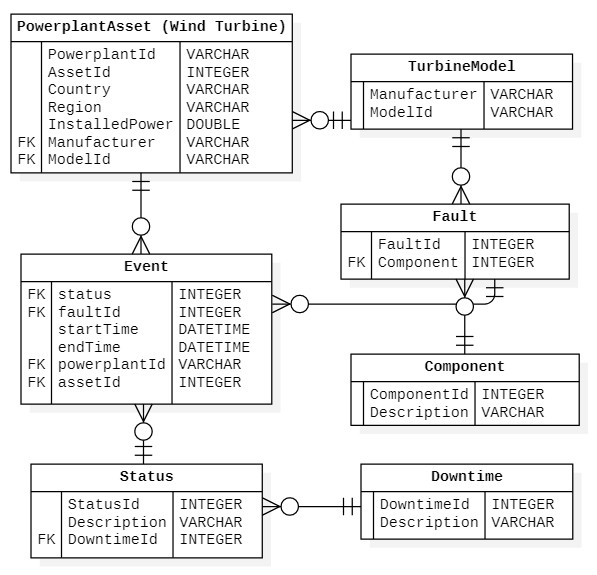
\includegraphics[scale=0.7]{Chapters/Figures/methodology_fig10.png}
	\caption{RMS Data Model of Data Acquisiton Entities: It represents all the entities that are involved in the data acquisition process and the storage of failure events.}
	\label{fig:Figuras_Tree_silhouettes-vectorial}
\end{figure}

Data from assets, allows us to understand the values of a certain asset during a time interval. In figure 5.2, we have the representation of all the entities that are involved in the calculation and storage of the data that the RMS CGI acquires from the wind turbines.
This data can have two origins: real-time data from field signals, or post processing data that uses the previous ones to make some calculations as soon as it is received (for example, expected power in wind turbines is calculated using wind speed, neighbors data, besides other data).
%Check if it's clear
The real-time data that is sent by the wind turbines are then received by a linked system that supports RMS CGI and that is responsible to aggregate them statistically in 10 minutes values (the number of minutes depends on each signal and client). This means, that in the statistical storage, we will have registered daily 144 values (one value per 10 minutes), each of these values represents the aggregation over the last 10 minutes, with the average value, minimum value, maximum of value and the standard deviation of the last 10 minutes of that signal for a specific timestamp.
To help in better structuring the signals comprehension, in RMS we use a term of tag that works as a string mask of the signal. In that way, it becomes easier to search for all the signals of multiple assets that concern a certain measure.

\begin{figure}[htbp]
	\centering
	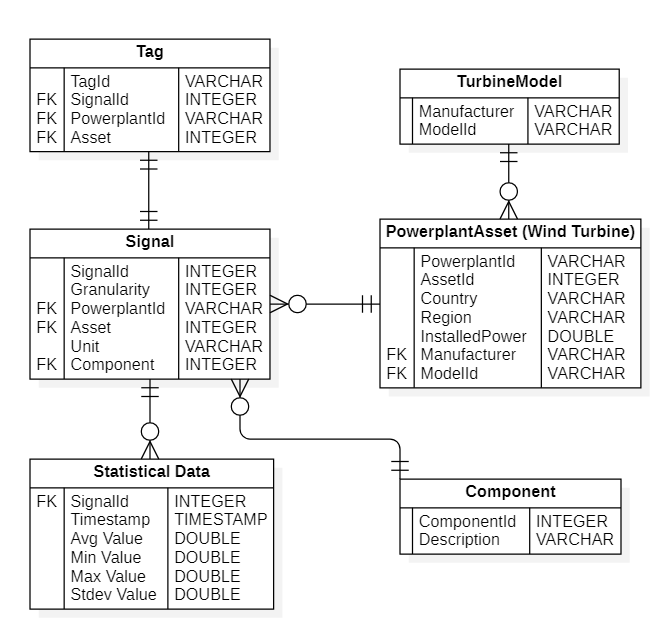
\includegraphics[scale=0.7]{Chapters/Figures/methodology_fig11.png}
	\caption{RMS Data Model of Storage of Data: It represents all the entities that are involved in the data acquisition, storage and statistical calculation of the data from the wind turbines.}
	\label{fig:Figuras_Tree_silhouettes-vectorial}
\end{figure}


\section{Dataset}
\label{sub:if_you_use_this_template} 
This thesis will focus on the data from CGI RMS concerning different parks in different locations of all Portugal, since the 5h March of 2021 until the end of that same year. This is the time interval of data that the current version of the RMS CGI has been running with all the configurations needed. Data that is stored in CGI RMS from previous years, came from a previous version of the CGI RMS system that was transitioned to the current system during this master thesis, and due to the fact that the processes of previous versions and current versions are not exactly the same, it has been decided that it shouldn't be used for this master thesis.

With the data available for those parks, a first analysis on the faults was made to understand two main questions in this thesis: 1) have we enough quality data to develop the machine learning models? 2) how can we predict the failure with the available monitoring data? 

\subsection{Have we enough data to train the machine learning models} 
\label{sub:if_you_use_this_template} 

As stated previously, in terms of data available in CGI RMS and classified as quality data, we have one major client portfolio of data that have different parks in different locations in Portugal.

This client provides data from 36 wind parks configured, with a total of 323 generators. These generators turbines have different manufacturers and models: a combination of 6 manufacturers and 13 turbine models compose these 323 generators. This client has configured 16,730 fault types and 31,970 different signals.
Considering, for example, July 2021 and one of the faults and wind turbine presented in Table 5.3, we have registered 184 events that concerns to that particular failure and wind turbine.

As presented earlier in the Data Structure section and in image Figure 5.1, we see that we can map to each failure event the component were the failure occurs and the energy loss and duration associated to that failure event, allowing us to classify the impact that the failure have in terms of financial loss and time to fix it. By knowing the exact moment when the failure was registered, we can correlate that data with the signals data from that component and asset, to understand how the wind turbine was behaving itself before the failure occurs, and to train the machine learning model to predict failures when those same or similar conditions occur.

%IMPROVEMENT: (PENSAR SE HA ALGO MAIS QUE POSSA COLOCAR)

\subsection{How can we predict the failure with the available monitoring data} 
\label{sub:if_you_use_this_template} 

To predict a failure, as any machine learning algorithm, we will provide samples of the dataset to train the algorithm. From all the signals available in the system, we selected a subset of some of the features that we will use as a starting point to train our model. The selection of each feature was supported by articles like \cite{OLD_41_WIND} [...] and by the opinion of CGI experts of renewable energy sources.

Each signal available depends on the manufacturer and model associated with the fault that is being study. So, to support the study of each fault, the features for each one might not be all the same and so this might be a factor that affects the performance of the model for the fault being predicted.

Despite this particularity of each model, a set of general features is selected for each fault. These features, displayed in Table 5.2 and mentioned in \cite{OLD_41_WIND} [...], are general information about the environment and the wind turbine.

\begin{table}[!ht]
    \centering
    \begin{tabular}{|l|l|p{0.35\linewidth}|l|}
    \hline
        Component & Unit & Description & Turbine Component \\ \hline
        WNAC\_WDSPD & M/S & Wind Speed & GENERAL / NACELLE \\ \hline
        WGEN\_W & KW & Active Power & GENERAL / GENERATOR \\ \hline
        WNAC\_WDDIR & DEG & Wind Direction & GENERAL / NACELLE \\ \hline
        WNAC\_EXTMP & DEGC & External Temperature / Temp outside / Temp. Ambient & GENERAL / NACELLE \\ \hline
        AIR\_DENSITY & KGM3 & Air Density & GENERAL \\ \hline
    \end{tabular}
    \caption{Wind Turbine General Information Signals. This signals exists for every wind turbines in the system.}
    \label{GeneralSignals}
\end{table}

We then selected some signals that are specific of each component of the fault itself. These features presented in Table 5.2, are features that exist for the majority of the manufacturers and models of the subset of faults and provide information specific of the component that they are connected to.
Some of these signals are mentioned by some articles of our literature that studied failures that affect some of these components also.

% DEPRECATED
%We then selected some signals that are specific of each component of the fault itself. These %features are specific for each manufacturer and model available, and provide us information %about the behaviour of the component associated with the fault.
%Some of these signals are mentioned by some articles like [ARTIGOS] that studied failures %that affect some of these components also.
%

\begin{table}[!ht]
    \centering
    \begin{tabular}{|l|l|p{0.27\linewidth}|p{0.15\linewidth}|p{0.15\linewidth}|}
    \hline
        Component & Unit & Description & ManufId & ModelId \\ \hline
        WGEN\_SPD & RPM & Generator Speed & ALL & ALL \\ \hline
        WTRM\_HYOILTMP & DEGC & Hydraulic oil temperature & F01 / F02 & N60 / N90 / V90 \\ \hline
        WTRM\_COOLTMP2 & DEGC & Temp cooling water return & F01 & N60 / N90 \\ \hline
        WTRM\_HYOILPRES & BAR & Hydraulic oil pressure & F01 / F02 / F06 & N90 / V90 / MM100 \\ \hline
        WTRM\_HYOILTMP & DEGC & Hydraulic oil temperature & F01 / F02 & N60 / N90 / V90 \\ \hline
        WNAC\_INTLTMP & DEGC & Nacelle Internal Temperature & F01 / F02 / F06 & N60 / V90 / MM100 \\ \hline
        WROT\_PTAGVALBL & DEG & Blade 1, actual value & ALL & ALL \\ \hline
        WROT\_ROTSPD & RPM & Rotor Speed & ALL & ALL \\ \hline
    \end{tabular}
    \caption{Wind Turbine Component Signals. These signals are specific for some manufacturers and models, and only exists for a subset of wind turbines. Provide information about a specific component.}
    \label{ComponentSignals}
\end{table}

In the last analysis on the features that we can use to provide more information about the wind turbines components, we made a specific analysis on the signals that we had available for each manufacturer and model. These signals are specific of some component of the wind turbine and are not available for all the wind turbines.
Since these signals are available depending on turbine manufacturer and model, this may lead that some machine learning models of failures of specific turbines contain features that have key data for the prediction of a failure and, consequently, perform better in terms of predicting those failures.
Some of the signals available are signals that have information about the current of the converter, temperature of several components and oil of these components, voltage of the transformer and generator. The complete list of signals is available in the Appendix1.

%TODO COLOCAR LISTA NO APPENDIX1!!!

Some signals that are mentioned in our literature and by CGI experts as important for the prediction of problems in wind turbines are vibration signals. Due to the fact that the wind turbine manufacturers don't provide them, we have to use other signals data that we have available, like temperature signals (gearbox oil temperature, etc.), that are considered to be one of the best alternatives to the vibration signals to predict failures in components, as said by CGI experts and in \cite{OLD_19_WIND}.

%MENTIONED IN THE PARAGRAPH ABOVE
%Some of these signals are considered key according to CGI experts of the %area, that indicate that some of these signals, specially the temperature %of the oil of a component, are fundamental to follow the state of a %component of the wind turbine and are the main candidates to replace the %subset of vibration signals, mentioned previosuly, and which the CGI RMS %have not available in their portfolio of signals.

\subsection{Dataset Structure} 
\label{sub:if_you_use_this_template} 

In terms of the dataset structure that will be introduced to the azure machine learning model, it will have the following columns. Some of these columns are only provided to have some metadata of the rows to be used for some intermediate steps (like the split of data).

\begin{enumerate}
    \item
TS (Datetime): provide information about the datetime of the row.
    \item
PowerplantId (String): the id of the wind turbine park.
    \item
AssetId (String): the id of the wind turbine.
    \item
Feature (one column per feature) (Double): the 10 min value of the feature for that particular timestamp. Some of the features column available are new variables created from others that are explained later in the Experiment Procedures-Feature Engineering chapter.
    \item
Fault (Boolean): indicates if the timestamp is in the sliding time window of failure. If it value is true, it means that the timestamp is inside the time window of one failure, and that the values of the feature of that same timestamp should be considered as indication that a failure will occur. Later, in Experiment Procedures chapter we will explain on how this column is built.
    \item
Failure Time (Boolean): indicates that in that timestamp a failure occurred. This column is specifically important in the evaluation of the final test dataset, to check if our machine learning model predicted with anticipation that failure time.
    \item
Fault Category (String): it was built to identify each failure event and to group them when each failure time is close to another failure time. In other words, indicates an id of a failure. The rows that do not correspond to a failure (indicating normal state of the wind turbine), will have an Fault Category value that indicates the next failure event. This means, that all the timestamps with a normal state of the wind turbine (Fault = 0) will have a Fault Category value equal to the next fault state of the wind turbine (Fault = 1).

\end{enumerate}

Each row of the dataset represents one timestamp of the wind turbine, and the correspondent values of the features and the fault state for that particular timestamp. In Figure 5.3, we can see an example of the dataset, with a set of rows starting in the 1st October 2021 at 07:20 to 10:30, with the values of the features ('WNAC EXTMP avg' and 'WGEN W avg'), the fault column that have the sliding time window of 72h in this case, and the failure event that occurred in the 08:50.

\begin{figure}[htbp]
	\centering
	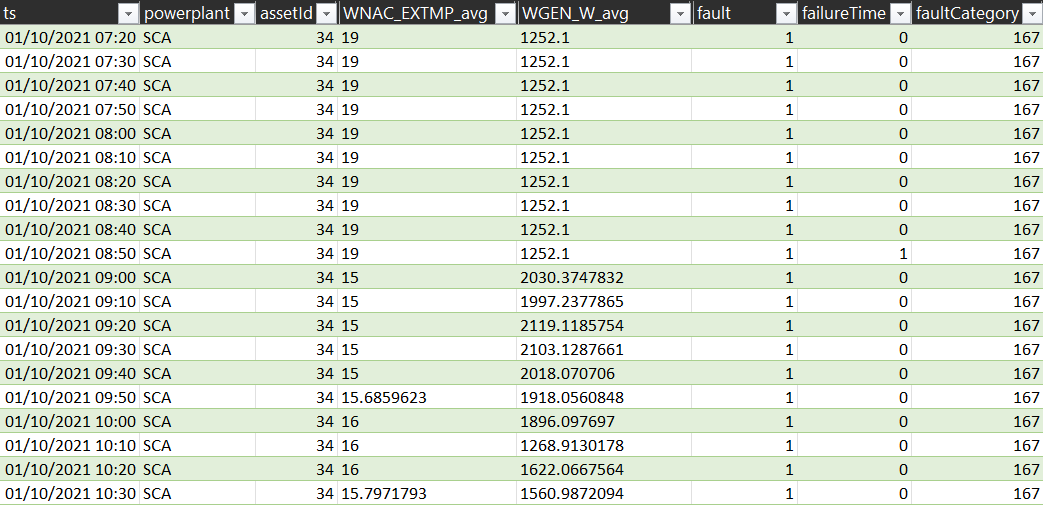
\includegraphics[scale=0.67]{Chapters/Figures/methodology_fig12.png}
	\caption{Example of the Dataset structure with all the columns: ts, powerplantId, assetId, two features ('WNAC EXTMP avg' and 'WGEN W avg'), fault, failure time and fault category. As explained previously in the fault category, rows prior to 07:20, that have the fault = 0, will have the same faultCategory, 167.}
	\label{fig:Figuras_Tree_silhouettes-vectorial}
\end{figure}

\section{Faults to Predict} 
\label{sub:if_you_use_this_template} 

In terms of the faults that were selected to be predicted, we started our analysis by ordering them with a first criteria of the number of events, thus meaning the faults that have more occurrences and consequently have more fault data to feed to our models. The second criteria was the total energy losses that the fault led to, thus meaning the direct impact in terms of lost of production and consequently the potential loss of revenues that the fault provoked to the client. We also filtered all the faults that are classified as alarms since these types of faults are not really faults, being alarms that the wind turbine provide to indicate a state of the wind turbine and that may be related to a maintenance or an alarm that is provoked by a component fault. These components faults are the ones that we will try to predict. The final selection criteria of the faults is to try to select the wider variety of manufacturers and model of faults and components, so that our study covers as many types of failures as possible. Our base number of top faults to study is around 10, but that number may vary according to the results of our analysis.

Initially when we start to analyze our approach of the best way to predict a specific failure in a portfolio of parks, we took the more generic approach possible. This means that we first though about joining in our dataset all the data of all the wind turbines of the same manufacturer and model in the prediction of a fault of that same manufacturer and model. A second approach, more restrict will be restrict only the wind turbines of the same park and that share the same manufacturer and model. Then after our first tests and after talking with the CGI experts and according to the feedback that a client of CGI RMS as given previously, we understand that this generic approach is not correct mainly due to this reason: even in the same park, each wind turbine varies from the others since each wind turbine is exposed to different external conditions (like wind direction), does not have always the same production (sometimes some wind turbines are limited in producing in comparison of wind turbines in the same park) and each component of the different wind turbines doesn't have the same level of degradation. 

%DEPRECATED BECAUSE IT IS NOT 100% CORRECT
%Secondly, if our model was built on a mixture of wind turbines each %prediction of a fault will only tell our client that a fault that is %concern a single component will occur on a possible subset of wind %turbines. This is not very useful for a maintenance point of view, since %the model does not indicate which specific wind turbines needs %maintenance.

So considering this point of view and the opinion of a client of CGI RMS, our final approach in terms of the range of variety that each model should be built, and justified by what has been told previously, was to build each model dataset and fit each model to predict a single failure of a specific wind turbine. This way our model will be more fitted to a wind turbine and the particular fault, thus resulting a prediction that will direct the client maintenance team to the particular component of the failure and to a particular wind turbine.

So, according to the filter and order criteria specified before, we obtain the following results presented in Table 5.3, that represent the top failures of the portfolio of parks that are going to be studied in this master thesis, in order to understand the correct approach to predict a failure in a wind turbine and thus, being these models the base model for the implementation of the Failure Prediction tool in CGI RMS.

The column 'Park', represents the id of a wind park. The column 'Asset', represents the id of the wind turbine for that park and the column 'FaultId', represents an id for the fault.

\begin{table}[!ht]
    \centering
    \begin{tabular}{|l|l|l|l|l|l|}
    \hline
        Park & Asset & faultId & nrEvents & energyLosses & duration \\ \hline
        SCA & 34 & 9112 & 573 & 28054.4697 & 4561720 \\ \hline
        SCA & 10 & 8487 & 325 & 348868.8745 & 1449668 \\ \hline
        BNE & 14 & 768 & 278 & 3476.3491 & 1022380,828 \\ \hline
        PAP & 35 & 8749 & 209 & 8510.8927 & 1699280 \\ \hline
        SCA & 28 & 8719 & 162 & 52329.0414 & 1862142 \\ \hline
        TMS & 6 & 14474 & 108 & 9563.8017 & 1157738 \\ \hline
        BNE & 18 & 768 & 102 & 800.9566 & 277801 \\ \hline
        CHF & 28 & 768 & 89 & 1760.2500 & 1093046 \\ \hline
    \end{tabular}
    \caption{Top Faults to be Analyzed}
    \label{TopFaultsTable}
\end{table}

After selecting the top faults, while the analysis was being made we decide to include for the same faults, some wind turbines which have a lower number of occurrences of faults events in order to understand if our model can have a similar power of prediction in case of wind turbines that have a substantial lower number of fault events. This subset of faults are presented in Table 5.4.

\begin{table}[!ht]
    \centering
    \begin{tabular}{|l|l|l|l|l|l|}
    \hline
        Park & Asset & faultId & nrEvents & energyLosses & duration \\ \hline
        PLS & 9 & 140 & 45 & 635.9669 & 556990 \\ \hline
        CHF & 15 & 367 & 19 & 65772.6703 & 478232,528 \\ \hline
        PCA & 7 & 140 & 81 & 1805.2607 & 733797 \\ \hline
    \end{tabular}
    \caption{SubsetFaults}
    \label{Subset of Faults with less occurences that are going to be analyzed}
\end{table}

According to the information of the signals available, provided in the dataset section, and the faults selected previously, in the Appendix X we can see the complete set of features available for each fault. These features are based on the first analysis presented in Table 5.3 and Table 5.4 presented earlier in the Dataset section, in 'How can we predict the failure with the available monitoring data' subsection.

For each of the faults presented in Table 5.3 and Table 5.4, we did an analysis on its distribution per month in order for us to understand the predictions that we should expect in each dataset used for training, validation and testing. That distribution information is presented in Table 5.5 and Table 5.6. In the experiment procedures section we will get into more detail in this step of distribution of the faults per each dataset.

\begin{table}[!ht]
    \centering
    \begin{tabular}{|l|l|l|l|l|l|l|l|}
    \hline
        Park & Asset & faultId & mar/21 & apr/21 & may/21 & jun/21 & jul/21 \\ \hline
        SCA & 34 & 9112 & 0 & 0 & 27 & 99 & 184 \\ \hline
        SCA & 10 & 8487 & 0 & 0 & 38 & 237 & 6 \\ \hline
        BNE & 14 & 768 & 0 & 5 & 31 & 217 & 6 \\ \hline
        PAP & 35 & 8749 & 0 & 0 & 3 & 43 & 16 \\ \hline
        SCA & 28 & 8719 & 0 & 0 & 0 & 12 & 111 \\ \hline
        TMS & 6 & 14474 & 0 & 0 & 4 & 2 & 58 \\ \hline
        BNE & 18 & 768 & 0 & 0 & 0 & 0 & 0 \\ \hline
        CHF & 28 & 768 & 0 & 0 & 0 & 0 & 0 \\ \hline
        CHF & 24 & 434 & 1 & 4 & 2 & 18 & 4 \\ \hline
        PAP & 22 & 8749 & 0 & 0 & 0 & 4 & 0 \\ \hline
        PLS & 9 & 140 & 0 & 0 & 2 & 14 & 9 \\ \hline
        CHF & 15 & 367 & 3 & 1 & 0 & 1 & 2 \\ \hline
        PCA & 7 & 140 & 0 & 0 & 1 & 7 & 7 \\ \hline
    \end{tabular}
    \caption{Faults Distribution per Month (March to End of July 2021)}
    \label{FaultsDistribitutionMarJun21}
\end{table}

\begin{table}[!ht]
    \centering
    \begin{tabular}{|l|l|l|l|l|l|l|l|}
    \hline
        Park & Asset & faultId & aug/21 & sep/21 & oct/21 & nov/21 & dec/21 \\ \hline
        SCA & 34 & 9112 & 139 & 78 & 44 & 2 & 0 \\ \hline
        SCA & 10 & 8487 & 2 & 4 & 10 & 8 & 0 \\ \hline
        BNE & 14 & 768 & 4 & 2 & 0 & 13 & 0 \\ \hline
        PAP & 35 & 8749 & 5 & 118 & 12 & 12 & 0 \\ \hline
        SCA & 28 & 8719 & 26 & 13 & 0 & 0 & 0 \\ \hline
        TMS & 6 & 14474 & 20 & 4 & 8 & 12 & 0 \\ \hline
        BNE & 18 & 768 & 0 & 85 & 17 & 0 & 0 \\ \hline
        CHF & 28 & 768 & 27 & 11 & 45 & 6 & 0 \\ \hline
        CHF & 24 & 434 & 4 & 7 & 0 & 4 & 0 \\ \hline
        PAP & 22 & 8749 & 0 & 16 & 26 & 0 & 0 \\ \hline
        PLS & 9 & 140 & 2 & 12 & 2 & 4 & 0 \\ \hline
        CHF & 15 & 367 & 4 & 3 & 5 & 0 & 0 \\ \hline
        PCA & 7 & 140 & 2 & 32 & 12 & 20 & 0 \\ \hline
    \end{tabular}
    \caption{Faults Distribution per Month (August to End of December 2021)}
    \label{FaultsDistribitutionAugDec21}
\end{table}


\section{Machine Learning Algorithms} 
\label{sub:if_you_use_this_template} 

In \cite{OLD_15_WIND} \cite{40_WIND} \cite{OLD_36_SOLAR}, it was studied, in a theoretical way, several possibilities of machine learning algorithms that are more adequate to achieve our main goal: the prediction and classification of failures that may occur in a wind turbine asset.

In terms of wind turbine faults, using \cite{OLD_15_WIND} \cite{OLD_53_WIND} \cite{40_WIND} \cite{ML_Alg_Analysis}, \cite{ML_Data_processing} and according to the recommendation from the CGI Machine Learning experts and the limitations of the algorithms already provided to us by the Azure Machine Learning Studio, the machine learning algorithms that we will focus our thesis are: Two-Class Logistic Regression, Two-Class Support Vector Machine (SVM), Two-Class Neural Network, Two-Class Boosted Decision Tree, Two-Class Decision Forest.

The machine learning algorithms will be used, with a dataset that contains the measures mentioned before for each fault and the other columns mentioned previously in the Dataset section. The target feature that will be used to fit our model is the column fault, mentioned earlier in the dataset section.
The main idea with this master thesis is to investigate and implement several machine learning models, each one with the function of predicting a single fault type of a wind turbine and being fitted for particular sliding time window parameter (explained later in this section), so that it can provide to the client which component of the specific wind turbine will fail and anticipate a preventive maintenance to minor the damage of a potential failure.
Another important goal of our models performance is to prioritize the minimization of false positives in comparison with predicting the maximum of true positives possible since we want our model to be reliable and not lead to maintenance's that are not needed.


\subsection{Classification Algorithms Studied} 
\label{sub:if_you_use_this_template} 

\subsubsection{Two-Class Logistic Regression}
The logistic regression is, at heart, a regression model. Logistic regression can be used as a classifier with the "purpose of obtaining a decision hyperplane that separates different classes" \cite{FCT_AA}.
The logistic regression, uses a function, denominated as a cost function, that takes value between 0 and 1 and that tell us the probability of a certain value being from one class or another. Thus, it is more applicable to binary problems.
This classification algorithm is the simplest to implement of all four and so, and because it is more advised to be used in binary classifiers, it is a good candidate to be an algorithm used to investigate single failures instead of a combination of failures from the same component.

In terms of its implementation in Azure Machine Learning Studio, we have available two parameters:
\begin{enumerate}
    \item{Optimization tolerance}
"Specify a threshold value to use when optimizing the model. If the improvement between iterations falls below the specified threshold, the algorithm is considered to have converged on a solution, and training stops" \cite{AZURE_MACHINE_LEARNING}
    \item{L2 Regularization Weight}
"Regularization is a method for preventing overfitting by penalizing models with extreme coefficient values. Regularization works by adding the penalty that is associated with coefficient values to the error of the hypothesis" \cite{AZURE_MACHINE_LEARNING}
\end{enumerate}


\subsubsection{Two-Class SVM (Support Vector Machine)}
It is a binary classification learning algorithm where each data item is a point in a n-dimensional space (where n is the number of features provided) and the classification is performed by finding the hyperplane that differentiates the two classes. The support vectors are data points that are closer to the hyperplane and influence the position and orientation of this hyperplane. Using the support vectors, we maximize the margin of the classifier. \cite{SVM}

One of the key parameters of the SVM classifier is the kernel function that is used. The kernel function is a function that "give us the inner product of the transformed vectors as a function of the original vectors" \cite{FCT_AA}, meaning that it is the function that converts the input data space into a higher-dimensional space. The kernel function "takes two data points and calculates a distance score be-tween those. This score is higher for closer data points and vice versa." \cite{SVM}. The more popular and the kernel functions that we are going to study are Linear Function, Polynomial Function, Radial Basic Function (RBF) and Sigmoid Function.

The key parameters that should be study in order to find out the values that are more adequate to our dataset is gamma, that defines how far the influence of a single training example reaches and C, that behaves as a regularization parameter in the SVM, in terms of margin of acceptance for the decision surface (lower C values lead to allowing more errors).
It is a good algorithm when we have a high number of features having a disadvantage of being slow. It is suited for extreme case binary classification and when the classes are separable.
Due to all this presented earlier, it seems to be a good algorithm for cases of component failures, where we have a lot of signals from that component, and when the amount of data is not high, because of being slow when the data set has a high number of samples. If these component failures don't happen at the same time, meaning that they are separable, it is also a good candidate.

In terms of its implementation in Azure Machine Learning Studio, we don not have available the specification of which kernel function to use neither some parameters mentioned earlier. In the Microsoft documentation it is not specified which kernel function is used, so we cannot have the complete information of how this module is implemented in the built-in module made available in Azure Machine Learning Studio.
For configuration of the hyperparameters of this module, we have available two parameters:
\begin{enumerate}
    \item{Number of Iterations}
"Denotes the number of iterations used when building the model. This parameter can be used to control trade-off between training speed and accuracy." \cite{AZURE_MACHINE_LEARNING}
    \item{Lambda}
"Value to use as the weight for L1 regularization. This regularization coefficient can be used to tune the model. Larger values penalize more complex models." \cite{AZURE_MACHINE_LEARNING}
    \item{Normalize Features}
"Before training, data points are centered at 0 and scaled to have one unit of standard deviation." \cite{AZURE_MACHINE_LEARNING}
\end{enumerate}

\subsubsection{Two-Class Neural Network}
A neural network, is an algorithm based in deep learning, as presented before in the background section. As presented in the Azure Machine Learning Studio documentation \cite{AZURE_MACHINE_LEARNING}, "a neural network is a set of interconnected layers. The inputs are the first layer, and are connected to an output layer by an acyclic graph comprised of weighted edges and nodes. Between the input and output layers you can insert multiple hidden layers. (...) The relationship between inputs and outputs is learned from training the neural network on the input data. The direction of the graph proceeds from the inputs through the hidden layer and to the output layer. All nodes in a layer are connected by the weighted edges to nodes in the next layer.
To compute the output of the network for a particular input, a value is calculated at each node in the hidden layers and in the output layer. The value is set by calculating the weighted sum of the values of the nodes from the previous layer".

In terms of its implementation in Azure Machine Learning Studio, we have available two parameters:
\begin{enumerate}
    \item{Hidden Layer Specification}
"Type of network architecture to create." \cite{AZURE_MACHINE_LEARNING}. It value can only be a Fully connected layer, where we have one hidden layer, being connected with the output layer and the input layer.
    \item{Learning Rate}
"Define the size of the step taken at each iteration, before correction. A larger value for learning rate can cause the model to converge faster, but it can overshoot local minimal." \cite{AZURE_MACHINE_LEARNING}
    \item{Number of learning iterations}
"specify the maximum number of times the algorithm should process the training cases." \cite{AZURE_MACHINE_LEARNING}
    \item{The momentum}
"specify a weight to apply during learning to nodes from previous iterations" \cite{AZURE_MACHINE_LEARNING}
    \item{Shuffle Examples}
"shuffle cases between iterations" \cite{AZURE_MACHINE_LEARNING}
\end{enumerate}

\subsubsection{Two-Class Decision Forest Classifier}
Decision Forest algorithm is based on Decision Tree. Decision Tree is a type of supervised algorithm that starts with a node that receives all the input features and that splits recursively based on those features. It predicts the value of a variable by extracting simple rules from data properties and learning those rules. Each split at a node is chosen to maximize information gain minimize entropy.
 
In terms of the decision forest, it is an ensemble learning method, thus meaning, that relies on multiple models, fixing in each iteration the mistakes from the previous build model. "This particular implementation of a decision forest works by building multiple decision trees and then voting on the most popular output class" \cite{AZURE_MACHINE_LEARNING}. This module implementation, use in each iteration the same complete dataset but with different starting points.

In terms of its implementation in Azure Machine Learning Studio, we have available two parameters:
\begin{enumerate}
    \item{Resampling Method}
"Method used to create the individual trees". The methods available are Bagging, in which "each tree is grown on a new sample, created by randomly sampling the original dataset with replacement until you have a dataset the size of the original" and Replicate in which "each tree is trained on exactly the same input data. The determination of which split predicate is used for each tree node remains random and the trees will be diverse" \cite{AZURE_MACHINE_LEARNING}.
    \item{Number of Decision Trees}
"Maximum number of decision trees that can be created in the ensemble" \cite{AZURE_MACHINE_LEARNING}.
    \item{Maximum depth of the decision trees}
"Number to limit the maximum depth of any decision tree". It allows to increase the precision of the model, with the risk of leading to overfit. \cite{AZURE_MACHINE_LEARNING}
    \item{Minimum number of samples per leaf node}
"Indicate the minimum number of cases that are required to create any terminal node (leaf) in a tree". This way, it allows to control the threshold for creating new rules. \cite{AZURE_MACHINE_LEARNING}.
\end{enumerate}

\subsubsection{Two-Class Boosted Decision Tree}
As the two-class decision forest classifier, boosted decision tree is also a type of decision tree classifier. Boosting, is a method that combines many weak learners tree, by each tree learning from the previous one, thus making a strong classifier. "Predictions are based on the entire ensemble of trees together that makes the prediction" \cite{AZURE_MACHINE_LEARNING}.

In terms of its implementation in Azure Machine Learning Studio, we have available two parameters:
\begin{enumerate}
    \item{Maximum number of leaves per tree}
"Indicate the maximum number of terminal nodes (leaves) that can be created in any tree". It allows to increase the precision of the model, with the risk of leading to overfit. \cite{AZURE_MACHINE_LEARNING}
    \item{Minimum number of samples per leaf node}
"Indicate the number of cases required to create any terminal node (leaf) in a tree". This way, it allows to control the threshold for creating new rules \cite{AZURE_MACHINE_LEARNING}.
    \item{Learning Rate}
"Number between 0 and 1 that defines the step size while learning. (...) Determines how fast or slow the learner converges on the optimal solution" \cite{AZURE_MACHINE_LEARNING}.
    \item{Number of trees constructed}
"Indicate the total number of decision trees to create in the ensemble". \cite{AZURE_MACHINE_LEARNING}
\end{enumerate}

\subsubsection{Configurable Parameters}
For the previous presented algorithms, as enumerated we have a serious of parameters to configure. In the Table 5.7, we present all the parameters that were configured for the algorithms. Some parameters presented are a subset of values. These parameters are the ones that are going to be analyzed using the Tune Model Hyperparameter module, that correspond to the hyperparameters of the algorithms. The static parameter values were chosen by running in an initial version of the experiment, and choosing from the available values, the parameter value that lead to the best results.

\begin{table}[!ht]
    \centering
    \begin{tabular}{|l|l|}
    \hline
    \multicolumn{2}{|c|}{\Text{Two-Class Logistic Regression}} \\
    \hline
        Optimization Tolerance & 0.00001; 0.00000001 \\ \hline
        L2 Regularization Weight & 0.01; 0.1; 1.0 \\ \hline
    \multicolumn{2}{|c|}{\Text{Two-Class SVM }} \\
    \hline
        Number of Iterations & 1; 10; 100; 250; 500; 750 \\ \hline
        Lambda & 0.00001; 0.0001; 0.001; 0.01; 0.1 \\ \hline
        Normalize Features & False \\ \hline
    \multicolumn{2}{|c|}{\Text{Two-Class Neural Network}} \\
    \hline
        Hidden Layer Specification & Fully-connected case \\ \hline
        Learning Rate & 0.1; 0.2; 0.4; 0.6; 0.8 \\ \hline
        Number of learning iterations & 25,50,100,175,250 \\ \hline
        The momentum & 0 \\ \hline
        Shuffle Examples & True \\ \hline
    \multicolumn{2}{|c|}{\Text{Two-Class Decision Forest Classifier}} \\
    \hline
        Resampling Method & Bagging Resampling \\ \hline
        Number of Decision Trees & 1; 8; 16; 32 \\ \hline
        Maximum depth of the decision trees & 1; 16; 32; 64 \\ \hline
        Minimum number of samples per leaf node & 1; 4;  8; 16 \\ \hline
    \multicolumn{2}{|c|}{\Text{Two-Class Boosted Decision Tree}} \\
    \hline
        Maximum number of leaves per tree & 2; 8; 32; 64; 128; \\ \hline
        Minimum number of samples per leaf node & 1; 10; 25; 50 \\ \hline
        Learning Rate & 0.025; 0.05; 0.1; 0.2; 0.4; 0.6 \\ \hline
        Number of trees constructed & 20; 50; 100; 250; 500 \\ \hline
    \end{tabular}
    \caption{Machine Learning Algorithms Set of Parameters Configured in the Azure Machine Learning Studio Experiment}
    \label{MLAlghoritmsParameters}
\end{table}


\section{Experiment Procedures}

As presented previously, our main goal is to analyze the features transformations that should be made and build an experiment that can be used for the prediction of the failures of wind turbine. So for that, and according to the modules available in the Azure Machine Learning Studio, we designed an experiment that build several models, each with the same procedures only differing the machine learning algorithm, so that for each fault and wind turbine we can evaluate each model result and then choosing the best fit for the scope that is being predicted.

\subsection{Data Pre-Processing Procedures}

In order to prepare our data, some pre-processing on the measures data that we have available from the signals described earlier in Table 5.1 and 5.2 must be done. The procedures that we selected to build our experience were based in our literature like \cite{ML_Data_processing} \cite{39_WIND} \cite{N_3_WIND} \cite{OLD_41_WIND} \cite{N_4_WIND} \cite{MED_1} \cite{N_7_GENERAL} and according to the modules available in the Azure Machine Learning Studio \cite{AZURE_MACHINE_LEARNING}.

First, in our acquisition of the data we analyze if a feature have a high percentage of null values for the entire dataset. If that is the case, we remove the feature because it means that it doesn't have enough quality data and the machine learning algorithm can't have null rows. The next step is to remove the remaining rows that contain any feature with a null value. These steps guarantee that we have a dataset with no invalid rows or features so that the process of training and fitting the model have no errors.

Then we proceed to the feature engineering step, by "create new features from the given dataset or tweak existing features to extract more valuable information" \cite{ML_Data_processing}, as stated also in \cite{N_7_GENERAL} \cite{MED_1}. This procedure is called running summaries as named in \cite{MED_1}.

Other step that was already mentioned before is the use of a sliding time window. This is a procedure that is made "to expand the failure or target window. That is, make the dependent variable, not just the day the equipment failed but the (...) appropriate interval leading up to the failure" \cite{MED_1}. This mechanism is also mentioned in Table 2 of \cite{N_7_GENERAL}, with the column Failure and in \cite{OLD_19_WIND} and \cite{TDC_1} were is explained how this new column is generated. As stated in this last article, "one usually does not need to predict the lifetime very accurate, far in the future. Often the maintenance team only needs to know if the machine will fail ‘soon'". So in order to do this and as presented in next Figure 5.4, we will use a sliding time window (presented in the figure as 'Z' in the x axis) and we will going to label it as 1 to represent a failure. This way, our model will be fitted to learn that Z time before a failure occur, the values of each feature may represent a behaviour that will lead to the failure of the wind turbine.

%CHECK IF THAT IMAGE SHOULD BE REPLACED
\begin{figure}[htbp]
	\centering
	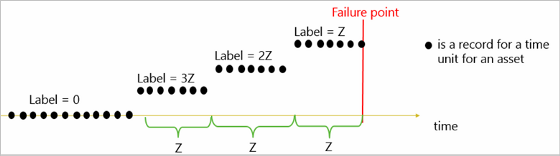
\includegraphics[scale=1.0]{Chapters/Figures/methodology_fig13.png}
	\caption{Sliding Time Window ...
	        \cite{TDC_1}}
	\label{fig:Figuras_Tree_silhouettes-vectorial}
\end{figure}

%METER O PORQUE DE TERMOS USADO O CHI-SQUARED BASEADO NUM SITE QUE VIMOS

The next refereed in \cite{ML_Data_processing}, \cite{N_4_WIND} and \cite{39_WIND} is the feature selection process where we extract only the useful and relevant features. This step "remove the problem of overfitting from your classification model". To do this procedure, we will use the Filter Based Feature Selection module available in Azure Machine Learning Studio, using the two-way chi-squared test. This is a "statistical method that measures how close expected values are to actual results (...) and indicates how far results are from the expected (random) result" \cite{AZURE_MACHINE_LEARNING}. "The (...) higher the Chi-Square value the feature is more dependent on the response and it can be selected for model training" \cite{TDC_ChiSquared}. The number of features that we choose to be selected was 30, and it was chosen by selecting on some of the best faults, several number of features and analyzing the results to check which number of features we obtained the best results of the model.

The next procedure is to split our dataset into the train, validation and test dataset, as mentioned in \cite{TDC_Train_Test_Split} \cite{TDC_TrainValidationTest}. In other articles in our literature, like \cite{Machine_Learning_Mistery_Train-Test-Split} \cite{ML_Data_processing} \cite{N_4_WIND} \cite{41_WIND} only use two-splits, the train and test dataset.
In our case, we will use a more custom split. In the beginning of the experiment we will use split our dataset from March 2021 to the 1st October 2021 and from that day to the end of the year of 2021. The first split will be used to train, fit and do a first evaluation of the model and the second split will be to get a total new dataset and simulate the behaviour of the model after being train and fitted, to understand it real score and real capacity for predicting faults.
In our first split (March 2021 to 1st October 2021), we will apply the Split Data module available in Azure Machine Learning Studio twice, so that we can achieve the three datasets that we pretend. We pretend to obtain 60\% for train, 30\% for validation and 10\% for testing. To obtain that, since we have to use the Split Data module twice, first we split with a fraction of 60\%, obtaining the train dataset, and on the remaining 40\%, we will split it into 70\%, thus giving approximately the percentages mentioned earlier for validation and test.

In terms of the type of split that we choose, we tried two approaches: first we did a randomized split, so that our data is completely unbiased in the rows chosen. Our second approach, by using a stratified split using the Fault Category column mentioned earlier, lead to best results and so was the approach selected.
As stated earlier, the failure event, have an id represented by the column fault category (presented earlier in dataset section). This failure event is multiplied by our sliding time window, as stated earlier. By splitting by the fault category, each dataset (the train, validation and test) contains part of each failure event and so our model is trained and evaluated using all the fault events available. This way, we guarantee that our model will use all the failure events in that timestamp, and thus learn the maximum number of patterns of the fault being study as possible. Our validation and test dataset will still evaluate if the model was correctly fitted to all the failure events since in these datasets it is present a portion of each failure event.
For example, if we have a sliding time window of 1 hour, our failure event is represented with 6 rows. With this split, our failure event is represented in the train dataset with 3 rows (approximately 60\%), that represents 3 timestamps, the validation will contain 2 rows of that failure (approximately 70\% of the remaining) and the test will contain 1 row of that failure (approximately the last portion).
Since we still have a second not used dataset to obtain our final results (data since October 2021 to the end of that same year), we still have available a complete new dataset to simulate our model behaviour and thus providing us a correct evaluation of our model.

%MAYBE PRESENT A CHART

If we do an analysis on the fault column for one of our faults that have the more number of fault events, and with the higher sliding time window of 72 hours (meaning that for each failure event, we will have 72*6 = 432 rows with fault = 1), for the column fault we have 9663 negatives (represented as 0, that means that the wind turbine was working correctly in that timestamp) and only 1996 positives, demonstrating that we have class imbalance since even with the sliding time window of 72 hours, only approximately 20\% of our rows represent a failure condition of the wind turbine.
"Class imbalance means one class is dominating and there are very few instances of the other class" \cite{ML_Data_processing}. This is normal in problems like the one that is being studied in this master thesis, since a wind turbine should stay most of it time running correctly and not with a specific type of failure.
In order to address this problem in our train dataset, we will synthesize new examples of the minority class, than in our case is the fault event. To do that, we will use the SMOTE (Synthetic Minority Oversampling Technique) module that exists in Azure Machine Learning Studio. SMOTE uses the k-nearest neighbor logic to build examples: "A randomly selected neighbor is chosen and a synthetic example is created at a randomly selected point between the two examples in feature space." [SMOTE].
After this process, we have a more balanced training dataset, having for the same fault mentioned before and after the SMOTE module, X negatives and Y positives.

% CHECK IF WE PUT  NEXT PARAGRAPH THIS BECAUSe OS PROFESSORES PODEM COMEÇAR A QUERER UMA ANALISE ESTATISTICA DETALHADA
%This number was selected from a previous analysis of the faults we were obtaining the best %results, and check the output of the Filter Based Feature Selection and module to check the %results of the two-way chi-squared test and the number of features that have  

\subsection{Train and Fit of the Model}
After all the pre-processing of the data, we are ready to feed to our machine learning algorithms mentioned before our dataset and creating our models. Each algorithm is available in Azure Machine Learning Studio and receives as input the train dataset. These modules configurations receive a parameter range, so that each parameter of each algorithm can receive a list of possible values that are then analyzed, using the Tune Model Hyperparameters module, and the validation dataset. 
The values selected for each parameter that were introduced were a varied list of values so that we can understand, for all the faults, for each algorithm which parameter values perform better on the overall of the faults.
In the previous presented Table 5.7, we can see for each algorithm which values were introduced for each parameter.

\subsection{Evaluation of the Model}
In terms of evaluating the model we based our evaluation in some standard metrics that are used in classification problems and that are mentioned in \cite{41_WIND} \cite{N_4_WIND} \cite{MED_1} [Classification]. These metrics are the Confusion Matrix, precision, recall and F1 Score.
To evaluate the dataset that simulates the behaviour of the dataset with a complete new dataset (with data since October 1st 2021 until the end of December 2021) which allow us to understand the true prediction power of our model, we use the metrics introduced earlier and we build a python script that evaluates the score model and evaluates if the failure events were correctly predicted inside the time window. This built metric is based according to \cite{MED_1} and the opinion of the CGI experts and is going to be explained later on.

Our standard metrics will be available by combining the Score Model module, which provides an table with the score of the model in each row, and the Evaluate Model module, that analysis the results of the Score Model and provide several metrics, in which are included all the ones mentioned.
The standard metrics will compare the Fault column from our dataset (the column that contains the failure event and the sliding time window rows) and the prediction output from our model.

\subsubsection{Standard Metrics}
The standard metrics mentioned earlier (Confusion Matrix, precision, recall and F1 Score) that we are going to use are common in evaluations of problems of binary classification.

\begin{enumerate}
    \item{Confusion Matrix}
Confusion matrix is a matrix that provide us four important terms: true positives (when the model predicts YES and the output is YES); true negatives (when the model predicts NO and the output is NO); false positives (when the model predicts YES and the output is NO); false negatives (when the model predicts NO and the output is YES).
As stated previously in this work, we have the priority of minimize as possible the false positives and try to have some true positives.
The confusion matrix terms forms the basis for the other types of metrics.

    \item{Precision}
It is the number of correct positive results divided by the number of positive results predicted by the classifier.

%METER EQUAÇÃO

    \item{Recall}
It is the number of correct positive results divided by the number of all relevant samples (all samples that should have been identified as positive).

%METER EQUAÇÃO

    \item{F1 Score}
Is calculated from the precision and recall. It's called the Harmonic Mean between the two and tries to find the balance between precision and recall, meaning that will tell how precise your classifier is, as well as how robust it is.
    
%METER EQUAÇÃO    
    
\end{enumerate}

\subsubsection{Final Evaluation Metric}
As presented in \cite{MED_1} and explained by the CGI experts, by using the column 'Fault', created in the data pre-processing step, to evaluate the performance of our model does not provide the correct result. This column reflects the failure event represented the Sliding Time Window multiplied by 6 (because each hour have 6*10 minute rows). For example, for a Sliding Time Window of 12 hours, we have each failure event represented 72 times. This may lead to cases where our model does not predict every single 1's in the fault column, but in the sliding time window interval, detects the amount of 1's enough to consider that in that interval it was detected the pattern that will lead to a failure of that fault type in that wind turbine. To understand and evaluate this capacity of the model, the most important column is the Failure Time column, that really indicates the timestamp where a fault occurred and the output from the python script that takes also into consideration the sliding time window interval of the dataset.

%TO CHECK THE COLUMN NAME
Our evaluation metrics, and considering our score model dataset which contains the structure presented in the first step of Figure 5.5, with the score of the model column, named Scored Model, is build following the presented steps:
\begin{enumerate}
    \item
Considering the table with the score model column, we will consider the sliding time window parameter. In this example, represented in the second step of Figure 5.5 we will consider 0.5 hours (30 minutes, that match with 3 timestamps).
    \item
On the dataset we build a new column, called 'Failure Prediction'. This column will be a Boolean (1 or 0), and it is going to indicate the real prediction of the model according to the interval considered in the previous step and the percentage threshold parameter.
The percentage threshold parameter is a percentage value, and indicates for a certain interval of analysis (the interval presented before), the percentage of predictions (1 values) in the interval that have to exists in order to consider that the end time of that interval represents a timestamp in which in the last 0.5 hours (our sliding time window parameter) the wind turbine is in failure conditions. The fill of that column is represented in the third step of Figure 5.5.
    \item
The last step is an iterative process that runs in all the rows. Each row evaluate the sliding time window before the timestamp in that row.
    \item
After the 'Failure Prediction' column is filled, we analyze the number of straight lines that have true values (represented as 1). Each set of straight lines represent an interval of prediction of the model. This means that from the start of that interval, to the end of that interval, the model predicted a failure event that might occur since the start timestamp of that interval to the end of that timestamp. These intervals are represented in Figure 5.6.
    \item
After these intervals are build up, we compare them to the timestamps in which we have a failure event, represented in our dataset with the column 'Failure Time'.
Then we evaluate with the same metrics as the Confusion Matrix: if the Failure Time is contained in one of these intervals, we classified as a True Positive; if the Failure Time is not contained in any of these intervals, it is considered a miss in prediction and so it counts to the False Negative; if the interval predicted does not contain any failure event, is a bad prediction and is considered an False Positive.
\end{enumerate}

\begin{figure}[htbp]
	\centering
	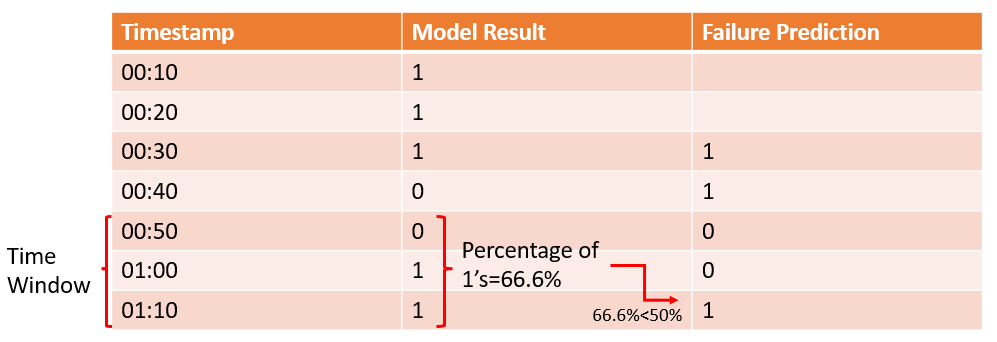
\includegraphics[scale=0.5]{Chapters/Figures/metric_example.png}
	\caption{Evaluation Script Example. The first column represents the timestamp, the second the prediction of the model and the third is the new column, created by the script that indicates, according to the interval and percentage threshold, which is the prediction of the model.}
	\label{fig:Figuras_Tree_silhouettes-vectorial}
\end{figure}

\begin{figure}[htbp]
	\centering
	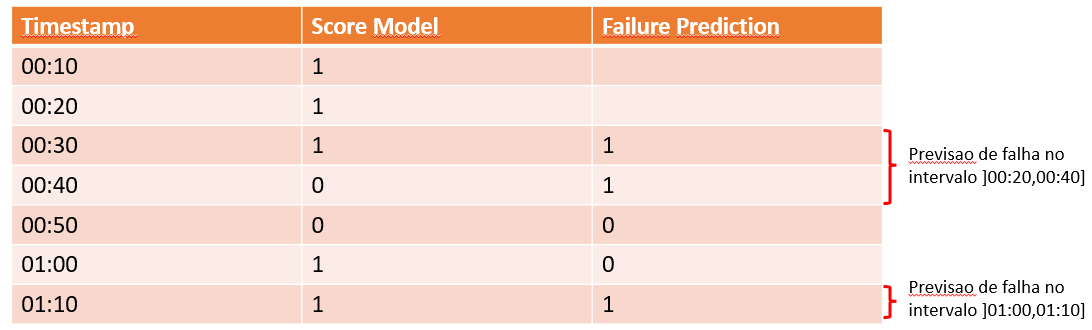
\includegraphics[scale=0.5]{Chapters/Figures/metric_example2.png}
	\caption{Evaluation Script Example 2. In this image and after the prediction of the model column ('Failure Prediction') is created, we have the predicted failure intervals represented.}
	\label{fig:Figuras_Tree_silhouettes-vectorial}
\end{figure}

%METER DIAGRAMA DE PROCESSO A EXPLICAR O PROCESSO COM UM EXCEL AO LADO (BASTA O PP)

\section{Conclusion} 
\label{sub:if_you_use_this_template} 
In this chapter, we present all the information, structures and methods that we are going to use to build our experiment and perform its evaluation. We started by presenting our data information that was used to build our dataset, the dataset structure, the scope of features that were used and then proceed to the scope of faults and wind turbines that was studied. Then, we advance to indicate which machine learning algorithms were used and present all the methods that are going to be used in our experiment. All these procedures and methods were selected according to the existing built-in modules in our main technology, the Azure Machine Learning Studio.